%%%%%%%%%%%%%%%%%%%%%%%%%%%%%%%%%%%%%%%%%%%%%%%%%%%%%%%%%%%%%%%%%%%%%%%%%%%%%
% IV Congresso Internacional de Biomassa
%%%%%%%%%%%%%%%%%%%%%%%%%%%%%%%%%%%%%%%%%%%%%%%%%%%%%%%%%%%%%%%%%%%%%%%%%%%%%

%%%%%%%%%%%%%%%%%%%%%%%%%%%%%%%%%%%%%%%%%%%%%%%%%%%%%%%%%%%%%%%%%%%%%%%%%%%%%
% CONFIGURAÇÕES GLOBAIS
%%%%%%%%%%%%%%%%%%%%%%%%%%%%%%%%%%%%%%%%%%%%%%%%%%%%%%%%%%%%%%%%%%%%%%%%%%%%%
\documentclass[12pt,ignorenonframetext,aspectratio=1610]{beamer}

\mode<presentation> {
  \usetheme[compress]{Boadilla}
  \setbeamercovered{transparent}
  \setbeamertemplate{page number in head/foot}[framenumber]
  \usefonttheme{structurebold}
  \definecolor{honeydew}{rgb}{0.94, 1.0, 0.94}
  \definecolor{green(munsell)}{rgb}{0.0, 0.66, 0.47}
  \definecolor{mygreen1}{rgb}{0.0, 0.5, 0.0}
  \definecolor{mygreen2}{rgb}{0.0, 0.5.5, 0.0}
  \definecolor{mygreen3}{rgb}{0.0, 0.6, 0.0}
  \definecolor{mygreen4}{rgb}{0.0, 0.4, 0.0}
  \definecolor{blond}{rgb}{0.98, 0.94, 0.75}
  \definecolor{bubbles}{rgb}{0.91, 1.0, 1.0}
  \definecolor{lightseagreen}{rgb}{0.13, 0.7, 0.67}
  \definecolor{midnightgreen(eaglegreen)}{rgb}{0.0, 0.29, 0.33}
  \definecolor{lightseagreen2}{rgb}{0.13, 0.8, 0.67}
  \definecolor{lightseagreen3}{rgb}{0.13, 0.6, 0.67}
  \definecolor{LightCyan}{rgb}{0.88,1,1}
  
  \setbeamercolor{structure}{fg=black}
  \setbeamercolor{titlelike}{parent=structure,bg=lightseagreen,fg=black}  \setbeamercolor{navigation symbols}{fg=green!90, bg=lightseagreen}
  \setbeamercolor{frametitle}{bg=midnightgreen(eaglegreen),fg=honeydew}
  \setbeamercolor*{palette primary}{bg=lightseagreen, fg = honeydew}
  \setbeamercolor*{palette secondary}{bg=lightseagreen3, fg = honeydew}
  \setbeamercolor*{palette tertiary}{bg=lightseagreen, fg = black}
}

%%%%%%%%%%%%%%%%%%%%%%%%%%%%%%%%%%%%%%%%%%%%%%%%%%%%%%%%%%%%%%%%%%%%%%%%%%%%%
% Novo ambiente para blocos
%%%%%%%%%%%%%%%%%%%%%%%%%%%%%%%%%%%%%%%%%%%%%%%%%%%%%%%%%%%%%%%%%%%%%%%%%%%%%
  \newenvironment{variableblock}[3]{%
  \setbeamercolor{block body}{#2}
  \setbeamercolor{block title}{#3}
  \begin{block}{#1}}{\end{block}}

% Imagem de plano de fundo
\usebackgroundtemplate%
{%
    
\includegraphics[width=\paperwidth,height=0.98\paperheight]{Fig/temp2.jpg}%
}

%%%%%%%%%%%%%%%%%%%%%%%%%%%%%%%%%%%%%%%%%%%%%%%%%%%%%%%%%%%%%%%%%%%%%%%%%%%%%
% Packages
%%%%%%%%%%%%%%%%%%%%%%%%%%%%%%%%%%%%%%%%%%%%%%%%%%%%%%%%%%%%%%%%%%%%%%%%%%%%%
\usepackage[portuguese]{babel} 
\usepackage[utf8]{inputenc} 
\usepackage{ragged2e} 
\usepackage[rightcaption]{sidecap}
\usepackage{graphicx} 
\usepackage{tikz} 
\usepackage{subfig}
\usepackage{multicol}
\usepackage[alf,abnt-emphasize=bf]{abntex2cite}
\usepackage{filecontents}
\usepackage{amsmath}
\usepackage{booktabs}
\usepackage{lscape}
\usepackage{pdflscape}
\usepackage{algorithmic}
\usepackage{adjustbox}
\usepackage[font=small,labelfont=bf]{caption}
\usepackage{wrapfig}
\usepackage{xcolor}
\usepackage[autostyle]{csquotes}
\usepackage{tikzsymbols}
\usetikzlibrary{shapes.geometric,arrows,positioning,mindmap,trees}
\usepackage{multimedia}
\usepackage{media9}
\usepackage{enumerate}
\usepackage{multicol}
\usepackage{smartdiagram}
\usepackage{color, colortbl}

%%%%%%%%%%%%%%%%%%%%%%%%%%%%%%%%%%%%%%%%%%%%%%%%%%%%%%%%%%%%%%%%%%%%%%%%%%%%%
\setbeamertemplate{headline}
{%
	\begin{beamercolorbox}[colsep=1pt]{upper separation line head}
	\end{beamercolorbox}
	\begin{beamercolorbox}{section in head/foot}
		\vskip1pt\insertnavigation{\paperwidth}\vskip1pt
	\end{beamercolorbox}%
	\begin{beamercolorbox}[colsep=1pt]{lower separation line head}
	\end{beamercolorbox}
}

% Customizando sumário
\setbeamertemplate{section in toc}{\hspace*{15em}\inserttocsectionnumber.~\inserttocsection\par}
\setbeamercolor{section in toc}{fg=white}
%%%%%%%%%%%%%%%%%%%%%%%%%%%%%%%%%%%%%%%%%%%%%%%%%%%%%%%%%%%%%%%%%%%%%%%%%%%%%
% Preâmbulo
%%%%%%%%%%%%%%%%%%%%%%%%%%%%%%%%%%%%%%%%%%%%%%%%%%%%%%%%%%%%%%%%%%%%%%%%%%%%%
\title[Aprendizado de Máquina e Biomassa Florestal]{{\normalsize Biomassa florestal: como construir e colocar em produção modelos de aprendizado de máquina usando a linguagem R?}}

\author[\textcolor{black}{Deivison V. Souza}]{\textbf{\textcolor{white}{Deivison Venicio Souza}\inst{}}}

\institute[Universidade Federal do Pará]
{\inst{}%
\textcolor{white}{	\scriptsize Universidade Federal Pará - UFPA \\ 
	\scriptsize Engenheiro Florestal, Me. Ciências Florestais \\ 
	\scriptsize Programa de Pós-graduação em Engenharia Florestal - UFPR \\
	\scriptsize Especialização Data Science \& Big Data (Em andamento) - UFPR \\
	\href{mailto:deivisonvs@ufpa.br}{\scriptsize (deivisonvs@ufpa.br)}	
	}}

\date[\today]{\textcolor{white}{\footnotesize \textbf{\Springtree[3] IV Congresso Internacional de Biomassa} \Springtree[3] \\ \textcolor{white}{\textbf{(Cibio)}}} \\
\vspace{.3cm} 
\textcolor{white}{25 a 27/06/2019 \\ Curitiba, PR}}

%%%%%%%%%%%%%%%%%%%%%%%%%%%%%%%%%%%%%%%%%%%%%%%%%%%%%%%%%%%%%%%%%%%%%%%%%%%%%
% LÂMINA 1
%%%%%%%%%%%%%%%%%%%%%%%%%%%%%%%%%%%%%%%%%%%%%%%%%%%%%%%%%%%%%%%%%%%%%%%%%%%%%
\begin{document}

\begin{frame}
 \titlepage
\end{frame}

%%%%%%%%%%%%%%%%%%%%%%%%%%%%%%%%%%%%%%%%%%%%%%%%%%%%%%%%%%%%%%%%%%%%%%%%%%%%%
% LÂMINA 2
%%%%%%%%%%%%%%%%%%%%%%%%%%%%%%%%%%%%%%%%%%%%%%%%%%%%%%%%%%%%%%%%%%%%%%%%%%%%%

\begin{frame}{Conteúdo}
 %\begin{multicols}{2}
  \tableofcontents
 %\end{multicols}
\end{frame}

%%%%%%%%%%%%%%%%%%%%%%%%%%%%%%%%%%%%%%%%%%%%%%%%%%%%%%%%%%%%%%%%%%%%%%%%%%%%%
% LÂMINA 3
%%%%%%%%%%%%%%%%%%%%%%%%%%%%%%%%%%%%%%%%%%%%%%%%%%%%%%%%%%%%%%%%%%%%%%%%%%%%%
\section{Biomassa de árvores}
\begin{frame}[t]{Biomassa de árvores}

\justifying
	
\begin{variableblock}{Definição}{bg=white,fg=black}{bg=black,fg=white}
\justifying
\vspace{.5cm}
\large{O termo “biomassa” se refere à massa dos componentes de uma árvore excluindo-se a água, isto é, a “\textbf{massa seca}” da árvore (BATISTA et al., 2014).}

\end{variableblock}	

\end{frame}

%%%%%%%%%%%%%%%%%%%%%%%%%%%%%%%%%%%%%%%%%%%%%%%%%%%%%%%%%%%%%%%%%%%%%%%%%%%%%
% LÂMINA 4
%%%%%%%%%%%%%%%%%%%%%%%%%%%%%%%%%%%%%%%%%%%%%%%%%%%%%%%%%%%%%%%%%%%%%%%%%%%%%
\begin{frame}[t]{Compartimentalização da biomassa de árvores}

	\begin{center}
		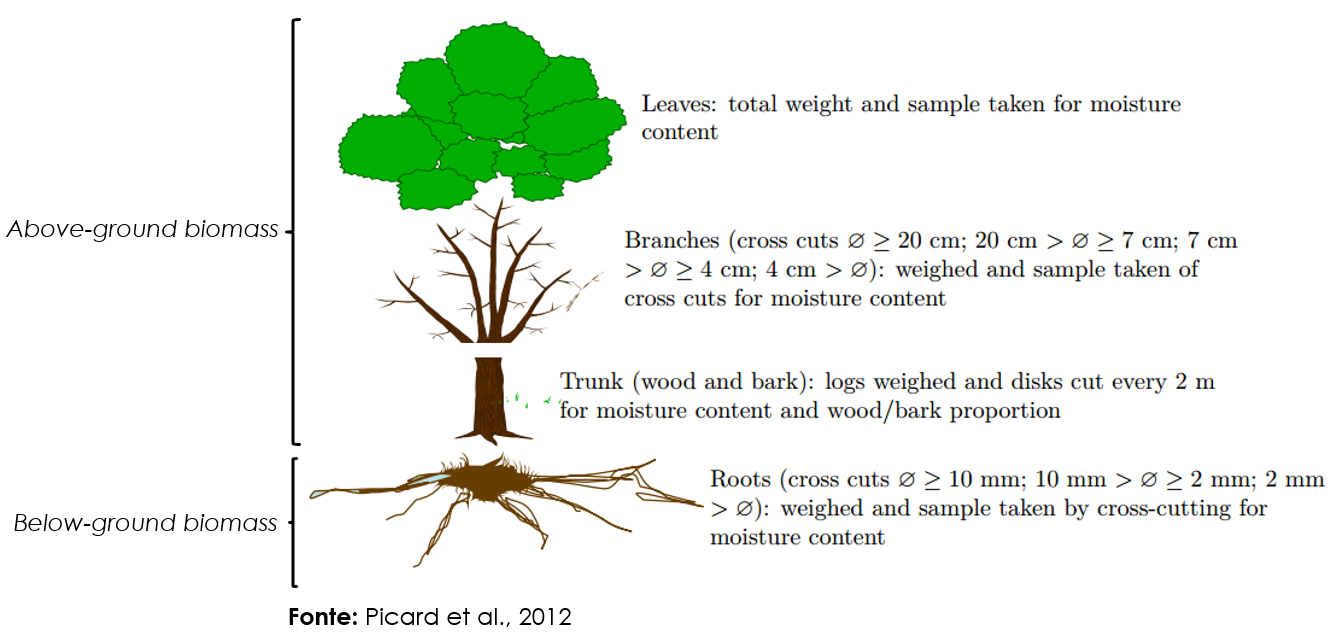
\includegraphics[scale=0.47]{Fig/Biomass3}
	\end{center}
	
\end{frame}

%%%%%%%%%%%%%%%%%%%%%%%%%%%%%%%%%%%%%%%%%%%%%%%%%%%%%%%%%%%%%%%%%%%%%%%%%%%%%
% LÂMINA 5
%%%%%%%%%%%%%%%%%%%%%%%%%%%%%%%%%%%%%%%%%%%%%%%%%%%%%%%%%%%%%%%%%%%%%%%%%%%%%
\begin{frame}[t]{Como quantificar a biomassa de árvores?}
		
\begin{center}
	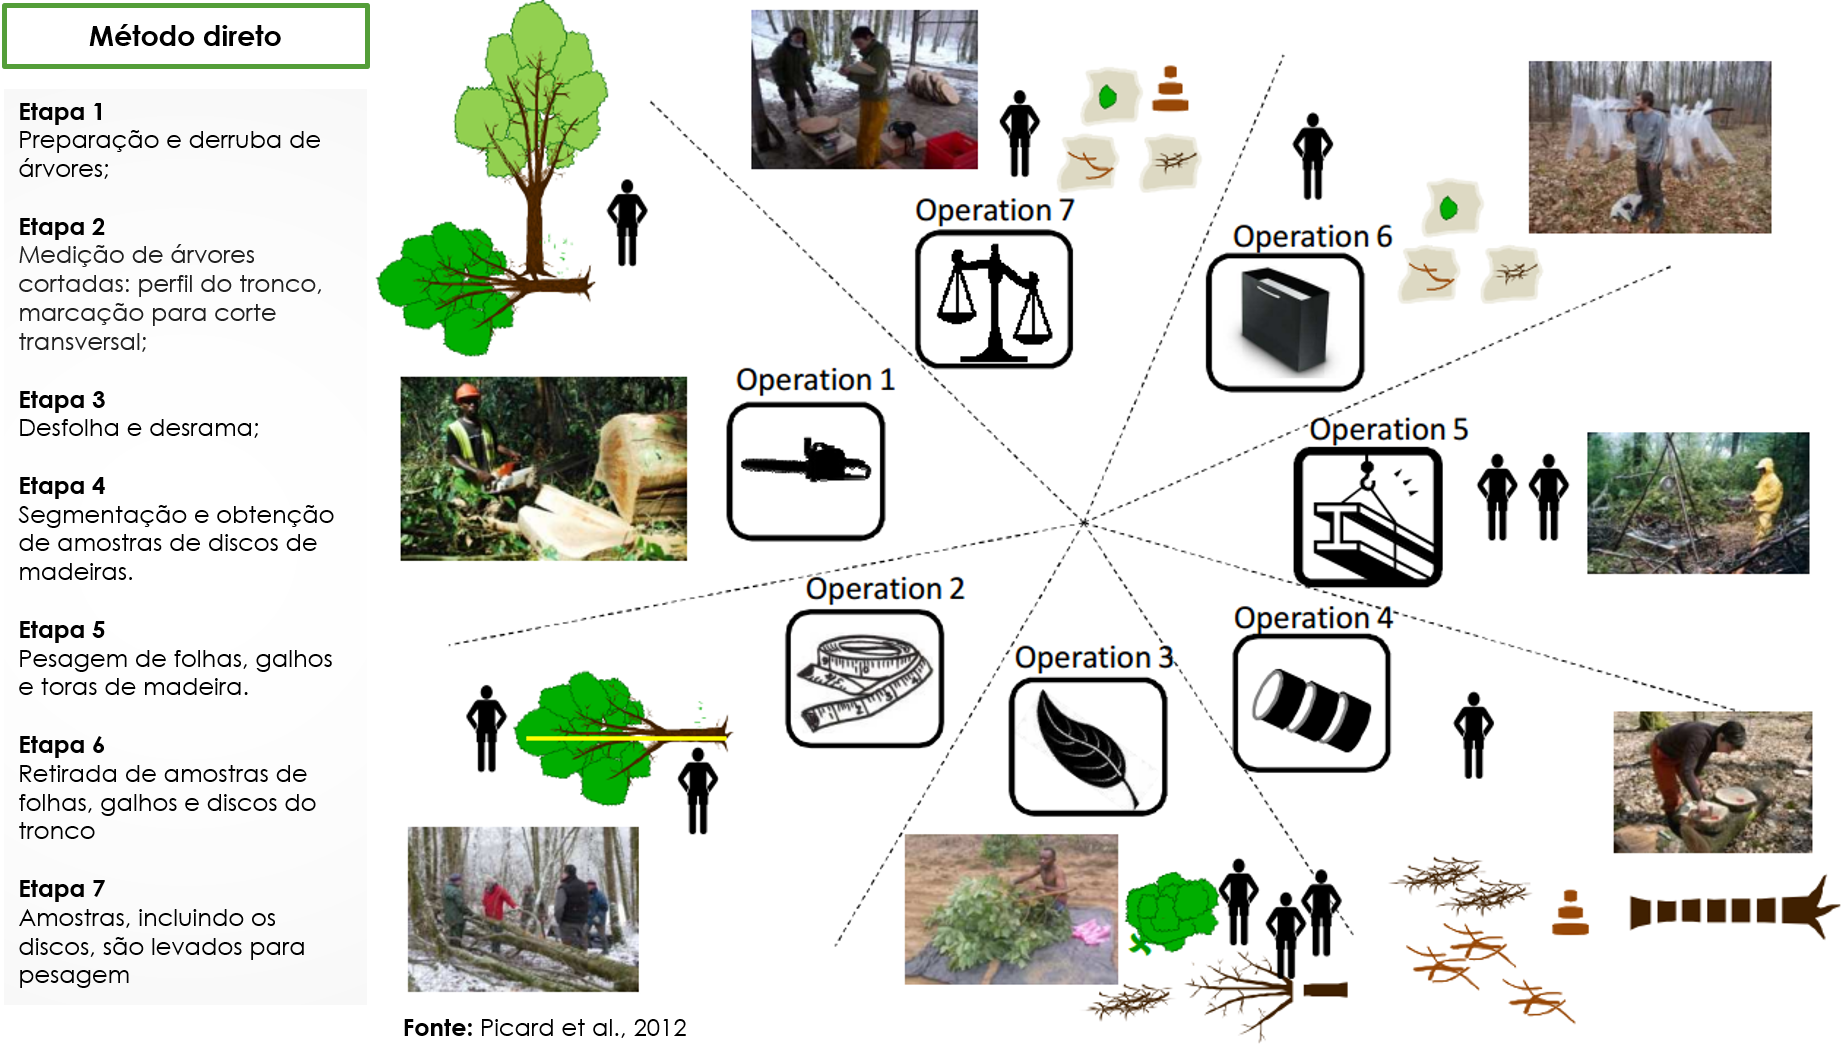
\includegraphics[scale=0.35]{Fig/Biomass2}
\end{center}
	
\end{frame}

%%%%%%%%%%%%%%%%%%%%%%%%%%%%%%%%%%%%%%%%%%%%%%%%%%%%%%%%%%%%%%%%%%%%%%%%%%%%%
% LÂMINA 6
%%%%%%%%%%%%%%%%%%%%%%%%%%%%%%%%%%%%%%%%%%%%%%%%%%%%%%%%%%%%%%%%%%%%%%%%%%%%%

\begin{frame}[t]{Aprendizado de Máquina}
    \begin{figure}[H]
        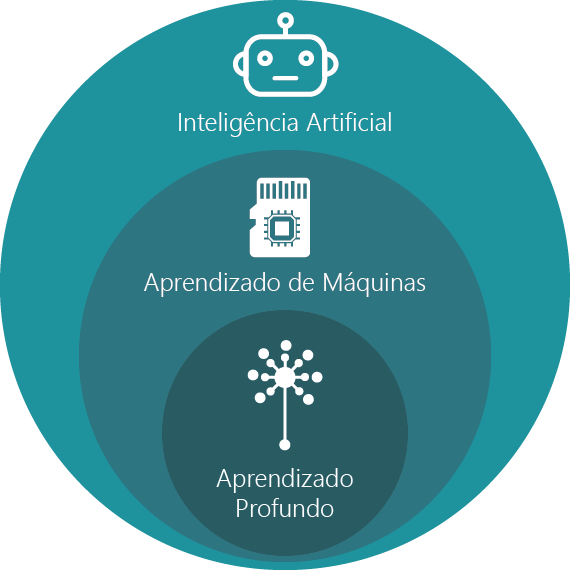
\includegraphics[width=7cm, height=6.5cm]{Fig/diag.png}
    \end{figure}
\end{frame}

%%%%%%%%%%%%%%%%%%%%%%%%%%%%%%%%%%%%%%%%%%%%%%%%%%%%%%%%%%%%%%%%%%%%%%%%%%%%%
% LÂMINA 7
%%%%%%%%%%%%%%%%%%%%%%%%%%%%%%%%%%%%%%%%%%%%%%%%%%%%%%%%%%%%%%%%%%%%%%%%%%%%%

\begin{frame}[t]{AM - Definição}
\transwipe
\hspace{5cm} \textcolor{white}{\textbf{Arthur Lee Samuel:} Termo} \textcolor{green}{``Machine Learning''}

\begin{variableblock}{Definição - Parafraseando Samuel (1959)}{bg=white,fg=black}{bg=black,fg=white}
\justifying
\vspace{.5cm}
\large{É um \textcolor{blue}{subconjunto de inteligência artificial} que frequentemente usa técnicas estatísticas para dar aos computadores a capacidade de \textcolor{blue}{``aprender'' com dados}, sem serem explicitamente programados.}
\end{variableblock}

\end{frame}

%%%%%%%%%%%%%%%%%%%%%%%%%%%%%%%%%%%%%%%%%%%%%%%%%%%%%%%%%%%%%%%%%%%%%%%%%%%%%
% LÂMINA 9
%%%%%%%%%%%%%%%%%%%%%%%%%%%%%%%%%%%%%%%%%%%%%%%%%%%%%%%%%%%%%%%%%%%%%%%%%%%%%

\begin{frame}[t]{Aprendizado supervisionado}
	
\begin{figure}[H]
	\centering
	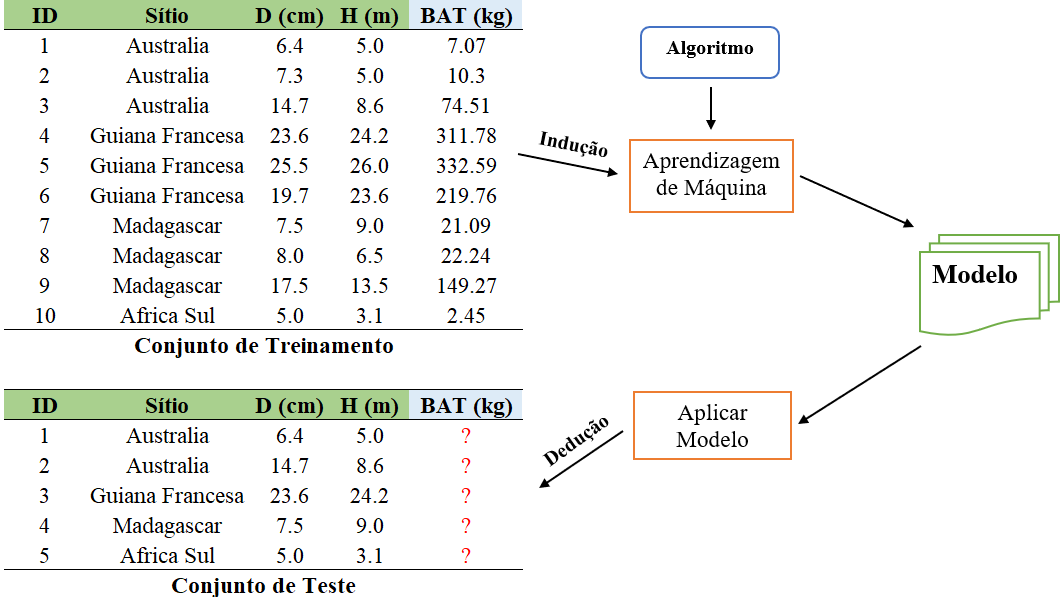
\includegraphics[scale=0.5]{Fig/Esquema.png}
\end{figure}
	
\end{frame}

%%%%%%%%%%%%%%%%%%%%%%%%%%%%%%%%%%%%%%%%%%%%%%%%%%%%%%%%%%%%%%%%%%%%%%%%%%%%%
% LÂMINA 10
%%%%%%%%%%%%%%%%%%%%%%%%%%%%%%%%%%%%%%%%%%%%%%%%%%%%%%%%%%%%%%%%%%%%%%%%%%%%%

\begin{frame}[t]{Um modelo de aprendizado de máquina}
	
\begin{figure}[H]
	\centering
	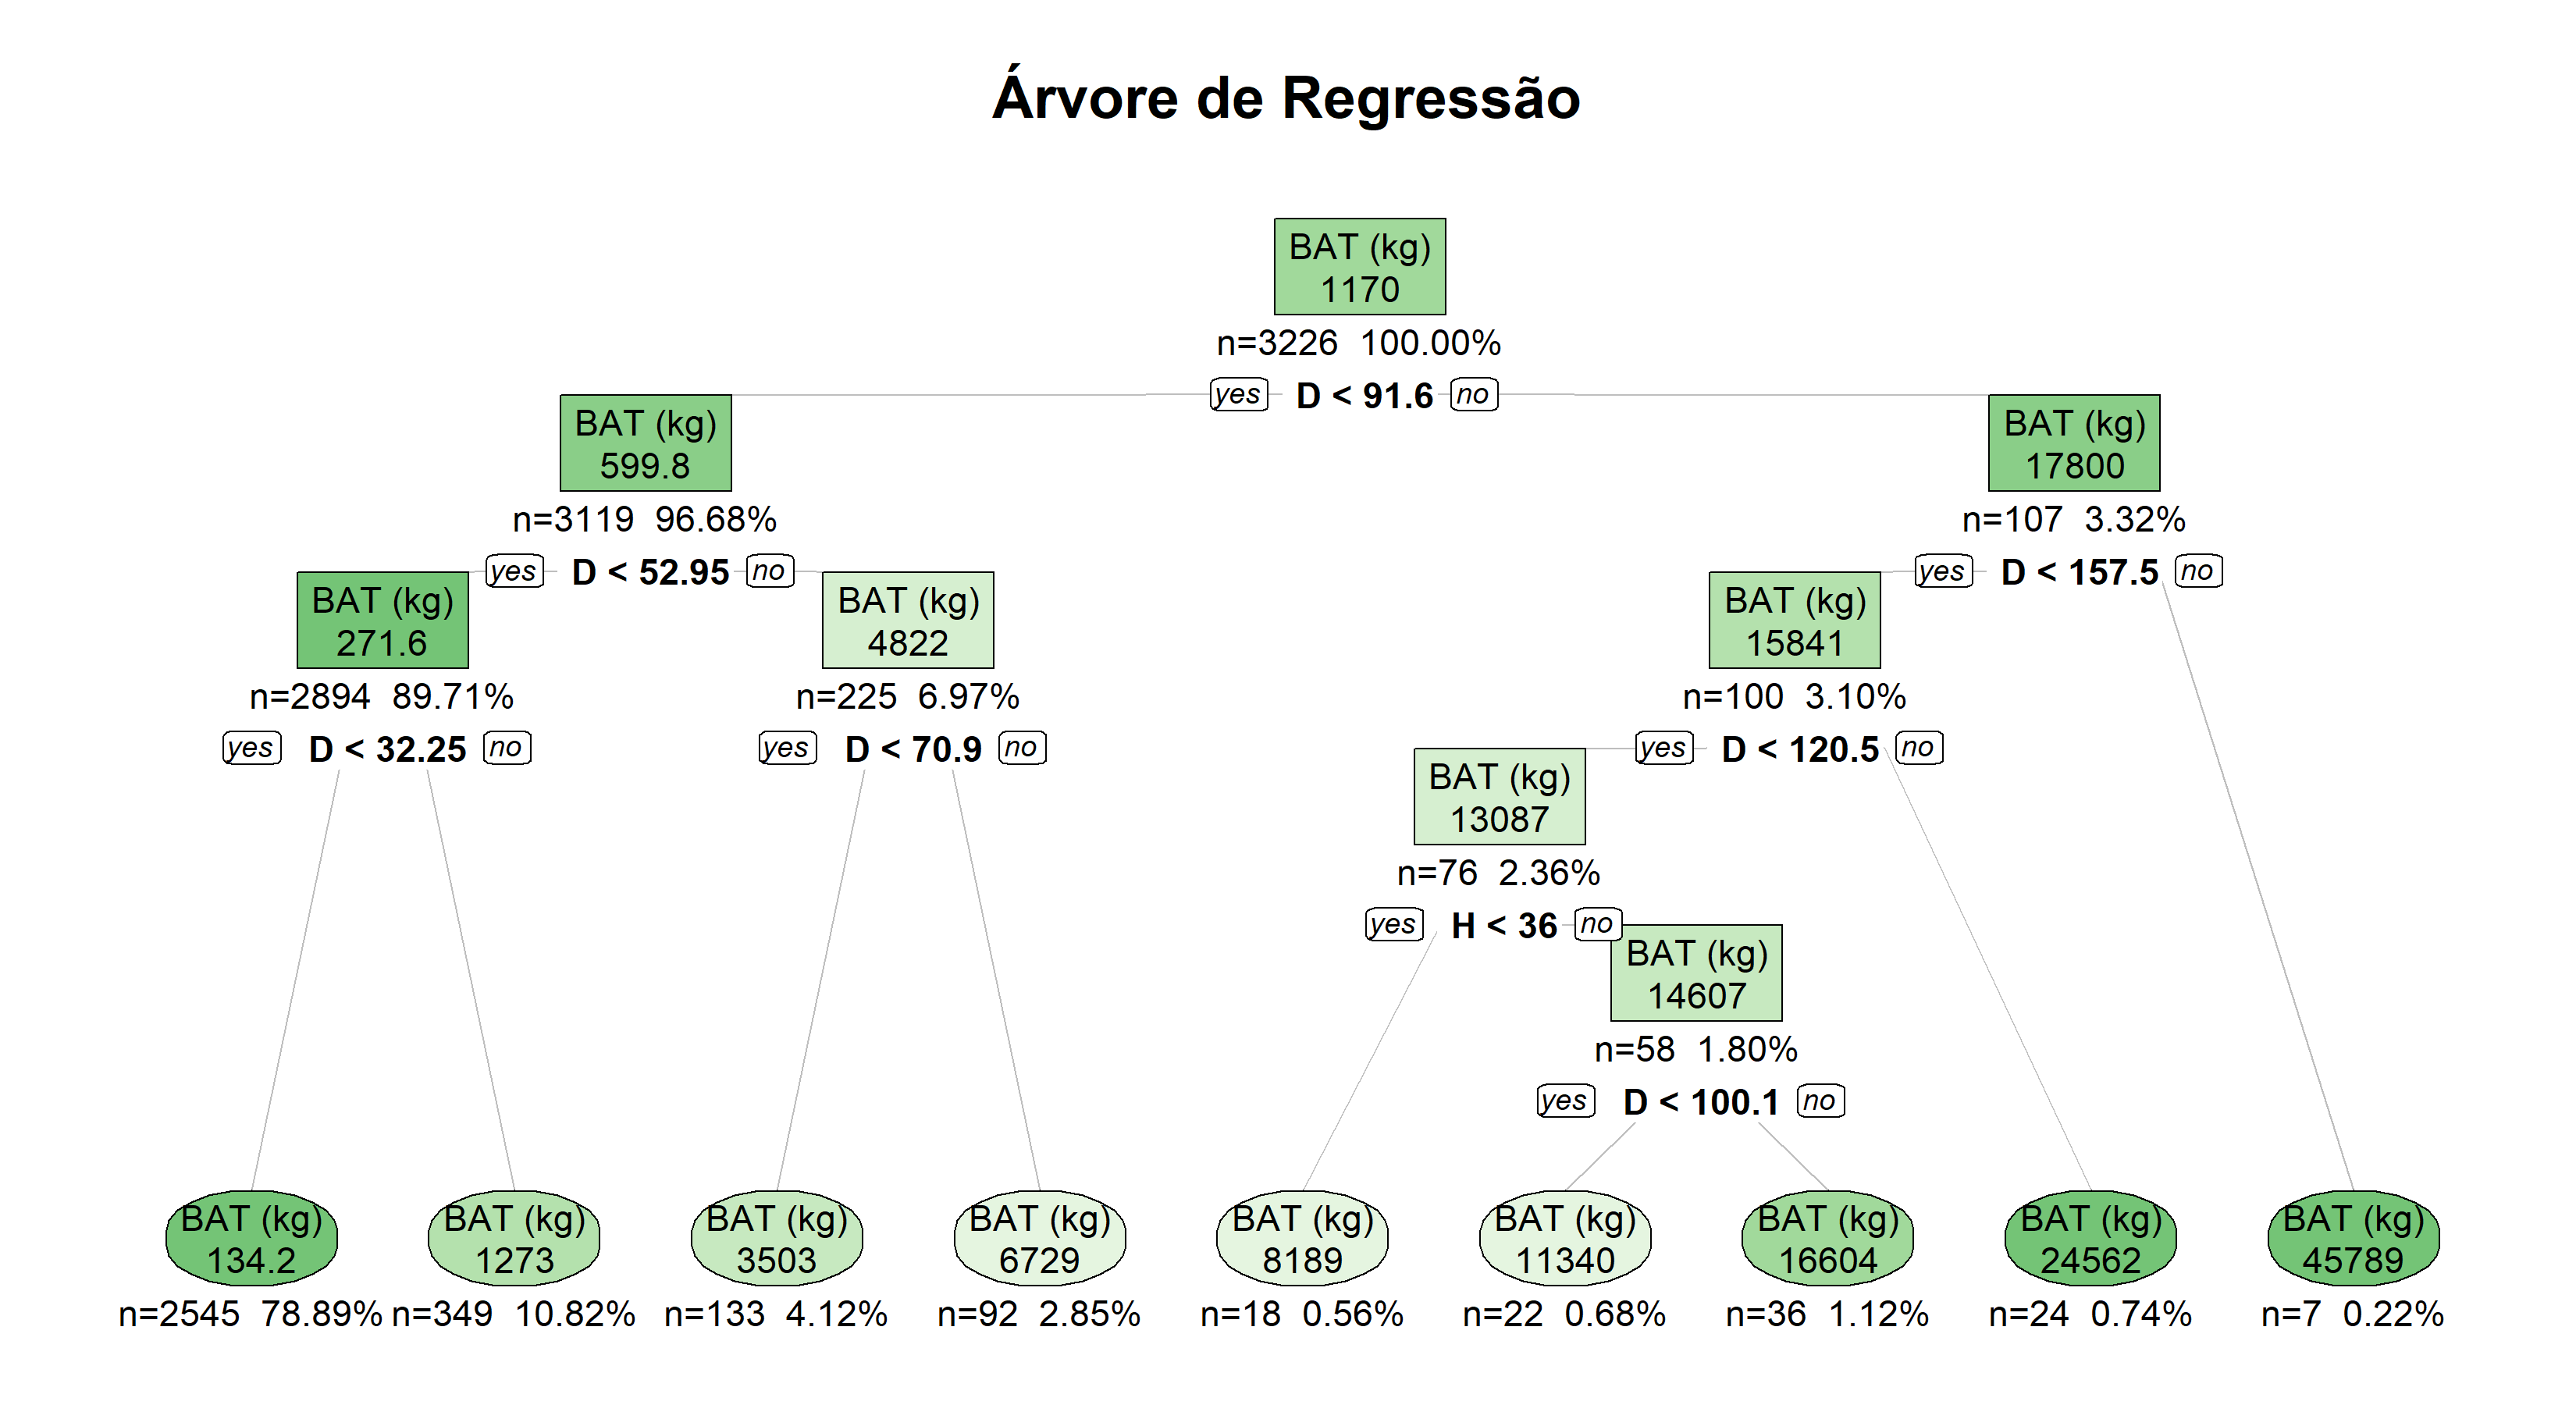
\includegraphics[scale=0.5]{Fig/CART.png}
\end{figure}
	
\end{frame}

%%%%%%%%%%%%%%%%%%%%%%%%%%%%%%%%%%%%%%%%%%%%%%%%%%%%%%%%%%%%%%%%%%%%%%%%%%%%%
% LÂMINA 11
%%%%%%%%%%%%%%%%%%%%%%%%%%%%%%%%%%%%%%%%%%%%%%%%%%%%%%%%%%%%%%%%%%%%%%%%%%%%%
\section{Aprendizado de Máquina no R}

\begin{frame}[t]{CRAN Task View}
	\justifying
	\hspace{5cm} \textcolor{white}{Até julho de 2018 existiam} \textcolor{green}{102 pacotes} \textcolor{white}{sobre AM \\ \hspace{5cm} publicados no CRAN Task View.}
	
	\begin{figure}[H]
		\centering
		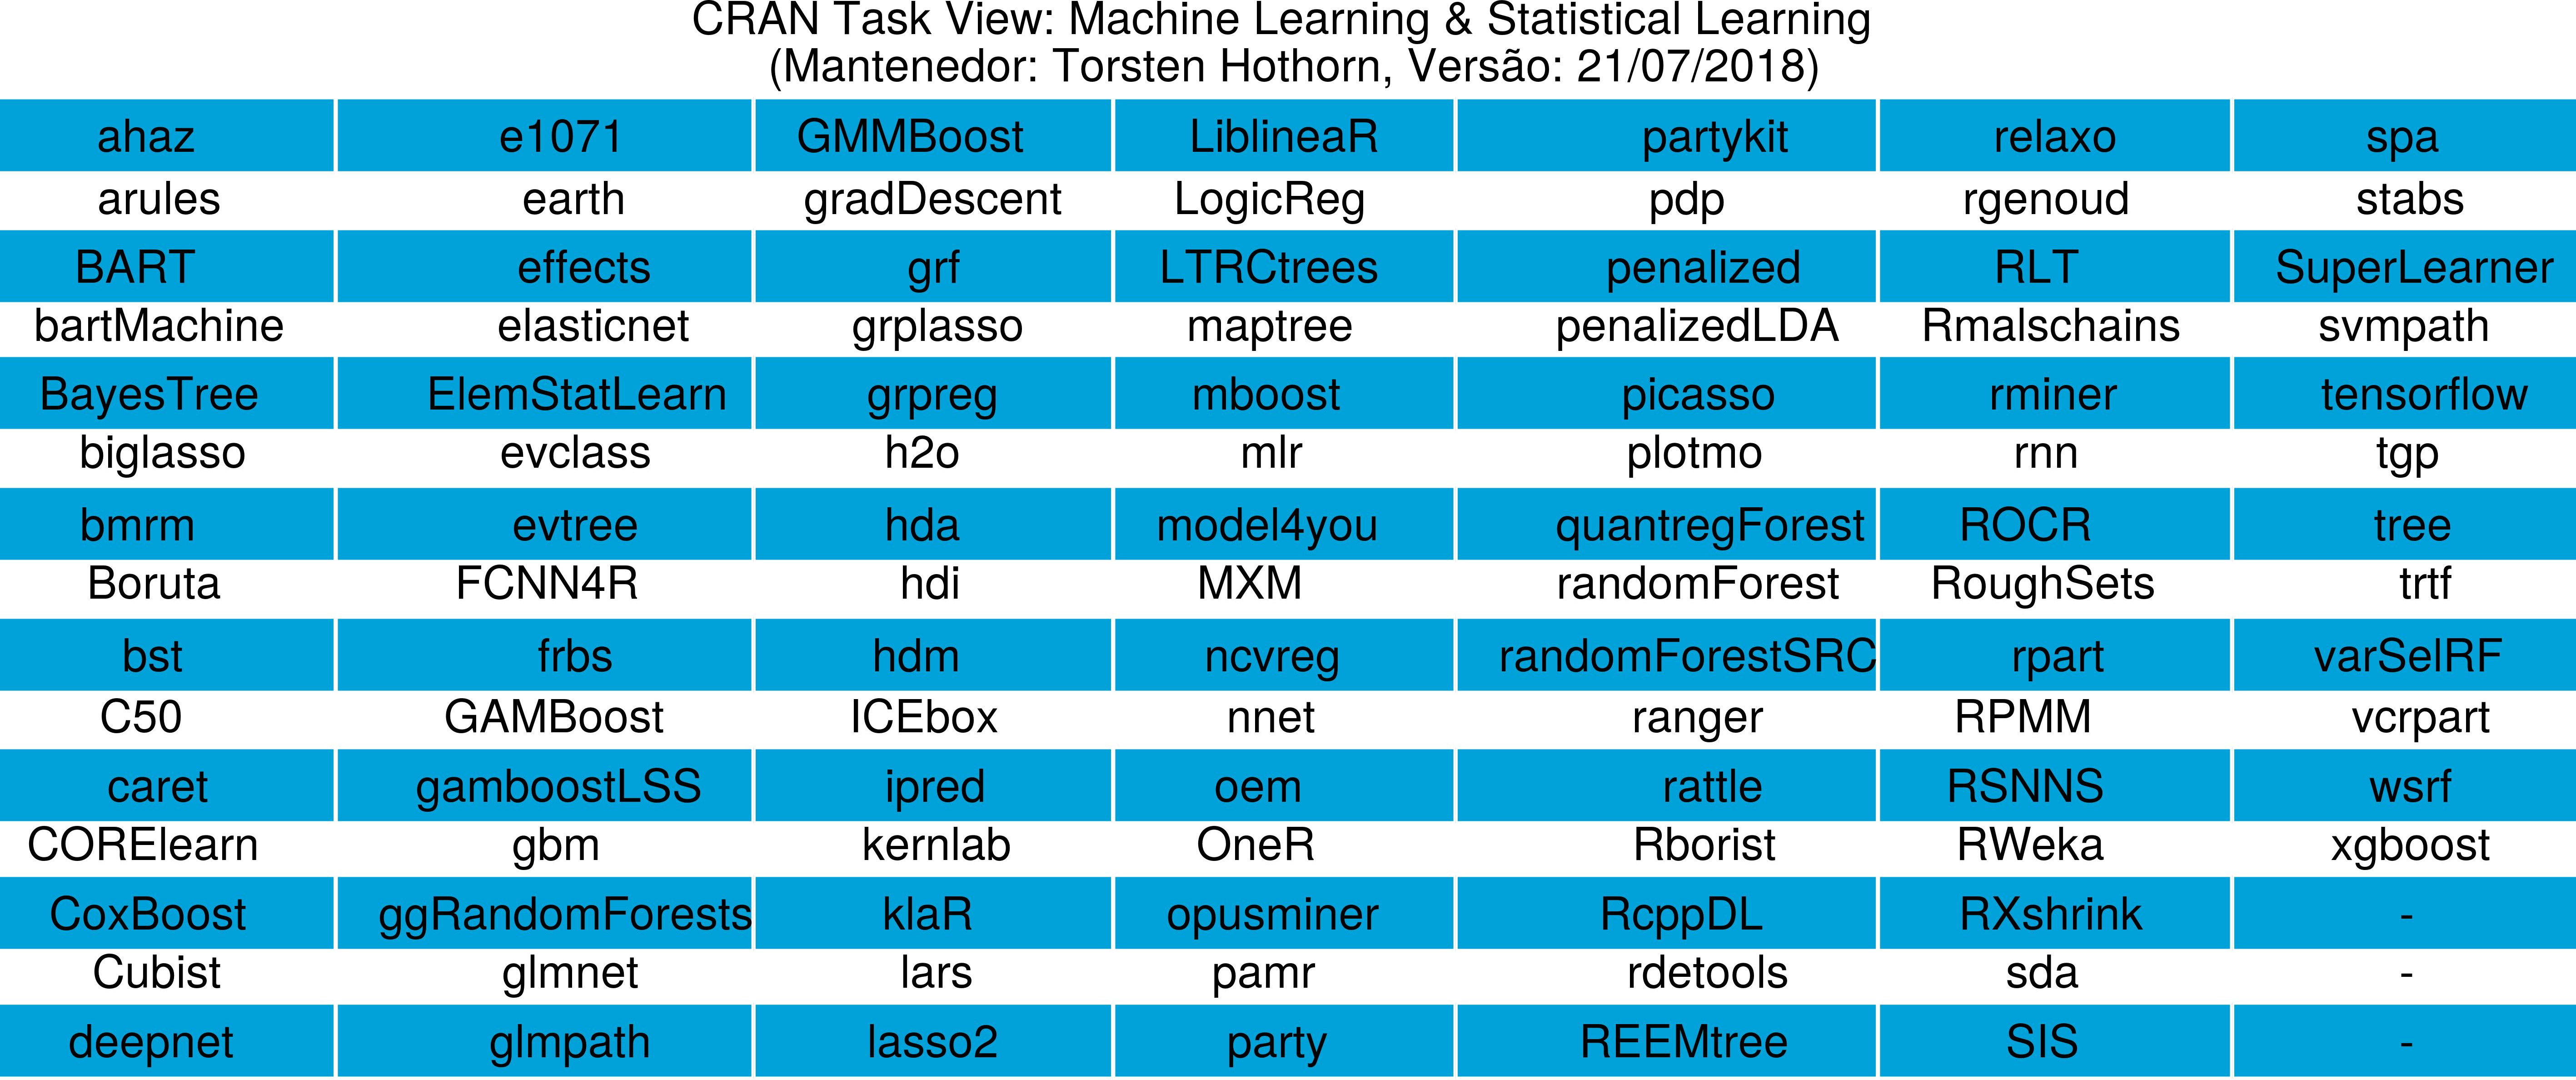
\includegraphics[scale=0.6]{Fig/Task2.jpeg}
	\end{figure}
	
\end{frame}

%%%%%%%%%%%%%%%%%%%%%%%%%%%%%%%%%%%%%%%%%%%%%%%%%%%%%%%%%%%%%%%%%%%%%%%%%%%%%
% LÂMINA 12
%%%%%%%%%%%%%%%%%%%%%%%%%%%%%%%%%%%%%%%%%%%%%%%%%%%%%%%%%%%%%%%%%%%%%%%%%%%%%
\begin{frame}[t]{TOP 20 - Downloads (último ano)}
	
	\begin{figure}[H]
		\centering
		\includegraphics[width=10cm, height=7cm]{Fig/dwl_year.jpeg}
	\end{figure}
	
\end{frame}	

%%%%%%%%%%%%%%%%%%%%%%%%%%%%%%%%%%%%%%%%%%%%%%%%%%%%%%%%%%%%%%%%%%%%%%%%%%%%%
% LÂMINA 13
%%%%%%%%%%%%%%%%%%%%%%%%%%%%%%%%%%%%%%%%%%%%%%%%%%%%%%%%%%%%%%%%%%%%%%%%%%%%%
\section{Pacote CAReT}

\begin{frame}[c]{}
	
	\begin{center}

	{\Huge \textcolor{white}{\textbf{Pacote}} \textcolor{green}{\textbf{CAReT}}} \\~\\
	
	{\Large\textcolor{white}{(}\textcolor{green}{\textbf{C}}\textcolor{white}{lassication} \textcolor{green}{\textbf{A}}\textcolor{white}{nd} \textcolor{green}{\textbf{Re}}\textcolor{white}{gression} \textcolor{green}{\textbf{T}}\textcolor{white}{raining)}} \\~\\
		
	\cite{kuhn2013applied, R-caret} \\~\\

	\hspace{1.5cm} \textcolor{white}{Constitui um conjunto de funções que tentam simplificar o processo de \\ \hspace{1.5cm} construção de modelos de aprendizado de máquina.} \\~\\
		
		
	\textbf{web page}: \href{https://topepo.github.io/caret/index.html}{https://topepo.github.io/caret/index.html}
	\end{center}
	
\end{frame}

%%%%%%%%%%%%%%%%%%%%%%%%%%%%%%%%%%%%%%%%%%%%%%%%%%%%%%%%%%%%%%%%%%%%%%%%%%%%%
% LÂMINA 14
%%%%%%%%%%%%%%%%%%%%%%%%%%%%%%%%%%%%%%%%%%%%%%%%%%%%%%%%%%%%%%%%%%%%%%%%%%%%%

\transwipe
\begin{frame}[c]{Pacote CAReT}

\hspace{5cm} \textcolor{white}{\large{Em termos gerais, o pacote} \textcolor{green}{CAReT} \textcolor{white}{possui \\ \hspace{5cm} ferramentas para:}}

\smartdiagramset{
 set color list={green!50, red!70, blue!50, gray!10, yellow!50},
 planet size=3cm,
 planet text width=3.5cm,
 planet font=\LARGE,
 satellite size=3.5cm, 
 satellite text width=4cm,
 satellite font=\LARGE,
 distance planet-text=0,
 %distance satellite-text=0,
 distance planet-satellite=6cm,
 /tikz/connection planet satellite/.append style={<-}
 } 
 \begin{center}
 \scalebox{0.4}{
 \smartdiagram[constellation diagram]{
  \textbf{Pacote CAReT},
    Seleção de recursos,
    Pré-processamento,
    Divisão de dados,
    Estimativa de importância das variáveis,
    Ajuste de modelo usando reamostragem
}}
  \end{center}

\end{frame}

%%%%%%%%%%%%%%%%%%%%%%%%%%%%%%%%%%%%%%%%%%%%%%%%%%%%%%%%%%%%%%%%%%%%%%%%%%%%%
% LÂMINA 15
%%%%%%%%%%%%%%%%%%%%%%%%%%%%%%%%%%%%%%%%%%%%%%%%%%%%%%%%%%%%%%%%%%%%%%%%%%%%%

\transwipe
\begin{frame}[t]{Pacote CAReT}
	\centering
		\begin{tabular}{@{}ll@{}}
			\toprule
			\rowcolor{LightCyan}
			\textbf{Função}                     & \textbf{Tarefa}  \\ \midrule
			\rowcolor{LightCyan}
			findCorrelation()      & Encontrar variáveis altamente correlacionadas \\
			\rowcolor{LightCyan}
			nearZeroVar()          & Identificar preditores com variância próxima de zero \\
			\rowcolor{LightCyan}
			\textcolor{magenta}{preProcess()}           & \textcolor{magenta}{Realizar pré-processamento} \\
			\rowcolor{LightCyan}
			\textcolor{magenta}{createDataPartition()}  & \textcolor{magenta}{Dividir aleatoriamente o conjunto de dados (estratificação)} \\
			\rowcolor{LightCyan}
			\textcolor{magenta}{train()}                & \textcolor{magenta}{Ajustar modelos preditivos utilizando reamostragem} \\ 
			\rowcolor{LightCyan}
			varImp()               & Estimar a importância das variáveis preditoras \\
			\rowcolor{LightCyan}
			resamples()            & Agrupar e visualizar os resultados da reamostragem \\
			\rowcolor{LightCyan}
			diff.resamples()       & Fazer inferências sobre diferenças de desempenho de modelos \\
			\rowcolor{LightCyan}
			confusionMatrix()     & Criar uma matriz de confusão \\
			\rowcolor{LightCyan}
			plotObsVsPred()       & Gerar gráfico de valores observados versus preditos \\ \bottomrule
		\end{tabular}
\end{frame}

%%%%%%%%%%%%%%%%%%%%%%%%%%%%%%%%%%%%%%%%%%%%%%%%%%%%%%%%%%%%%%%%%%%%%%%%%%%%%
%% LÂMINA 16
%%%%%%%%%%%%%%%%%%%%%%%%%%%%%%%%%%%%%%%%%%%%%%%%%%%%%%%%%%%%%%%%%%%%%%%%%%%%%
\begin{frame}[c]{Processo AMS - Simplificado}

\tikzstyle{decision} = [diamond, draw, fill=orange!30, 
    text width=4.5em, text badly centered, node distance=3cm, inner sep=0pt]

\tikzstyle{circle1} = [circle, draw, fill=green!20, text centered, radius = 5em]

\tikzstyle{block} = [rectangle, draw, fill=blue!20, 
    text width=6em, text centered, rounded corners, minimum height=4em]
    
\tikzstyle{line} = [draw, -latex',color=white]
\tikzstyle{line2} = [draw, -latex',color=green]

\tikzstyle{cloud} = [draw, ellipse,fill=red!20, node distance=3cm,
    minimum height=2em]

\tikzstyle{block1} = [rectangle, draw, fill=red!20, text width=8.3em, text centered, rounded corners, minimum height=1.5em]

\tikzstyle{block2} = [rectangle, draw, fill=red!20, text width=4.5em, text centered, rounded corners, minimum height=1.5em]

\tikzstyle{block3} = [rectangle, draw, fill=blue!20, 
    text width=8em, text centered, rounded corners, minimum height=4em]

\begin{tikzpicture}[node distance = 3.1cm, auto]

% Place nodes
    \node [circle1] (prob) {Problema};
    \node [block, right of=prob] (ide) {Obtenção de dados};
    \node [block, right of=ide] (pre) {Pré-processamento};
    \node [block, right of=pre] (def) {Definição do conjunto de treinamento};
    \node [block, right of=def] (sel) {Seleção de algoritmos};
    \node [block, below of=sel] (treino) {Aprendizado (tuning)};
    \node [block, left of=treino] (teste) {Avaliação no conjunto de teste};
    \node [decision, left of=teste] (dec) {Ok?};
    \node [block, left of=dec] (CR) {Classificador ou Regressor};
    \node [block1, above of=def,node distance=1.5cm] (cdp) {createDataPartition};
    \node [block2, above of=pre,node distance=1.5cm] (preP) {preProcess};
    \node [block2, below of=treino,node distance=1.5cm] (train) {train};
    
% Draw edges
    \path [line] (prob) -- (ide);
    \path [line] (ide) -- (pre);
    \path [line] (pre) -- (def);
    \path [line] (def) -- (sel);
    \path [line] (sel) -- (treino);
    \path [line] (treino) -- (teste);
    \path [line] (teste) -- (dec);
    \path [line] (dec) -- (CR);
    \path [line,dashed] (pre) -- (preP);
    \path [line,dashed] (def) -- (cdp);
    \path [line,dashed] (treino) -- (train);
    \path [line] (dec) -- node[near start]{Sim}(CR);
    \draw[line2,dashed] (dec) to[out=90,in=-90] (ide);
    \path [line2,dashed] (dec) -- node [near start]{Não}(pre);
    \draw[line2,dashed] (dec) to[out=90,in=-90] (def);
    \draw[line2,dashed] (dec) to[out=90,in=-150] (sel);
    
\end{tikzpicture}
\end{frame}

%%%%%%%%%%%%%%%%%%%%%%%%%%%%%%%%%%%%%%%%%%%%%%%%%%%%%%%%%%%%%%%%%%%%%%%%%%%%%
% LÂMINA 17
%%%%%%%%%%%%%%%%%%%%%%%%%%%%%%%%%%%%%%%%%%%%%%%%%%%%%%%%%%%%%%%%%%%%%%%%%%%%%
\begin{frame}[t]{Alguns algoritmos disponíveis}

\hspace{5cm}\textcolor{white}{\textbf{Total}: 238 algoritmos} \\~\\

\begin{adjustbox}{max width=\textwidth}
\begin{tabular}{@{}lllll@{}}
\toprule
\rowcolor{LightCyan}
\textbf{Modelo}          & \textbf{Método}   & \textbf{*Tarefa}    & \textbf{Pacote origem}       & \textbf{Hiperparâmetro} \\ \midrule
\rowcolor{LightCyan}
k-Nearest Neighbors     & knn               & C, R               & caret        & k                      \\
\rowcolor{LightCyan}
SVM with Linear Kernel  & svmLinear         & C, R   & kernlab      & C                      \\
\rowcolor{LightCyan}
Extreme Gradient Boosting
  & xgbTree        & C, R   & xgboost        & nrounds, eta, max\_depth                   \\
\rowcolor{LightCyan}
Multi-Layer Perceptron  & mlp               & C, R   & RSNNS        & size                   \\
\rowcolor{LightCyan}
Neural Network          & neuralnet         & R      & neuralnet    & layer1,layer2,layer3   \\
\rowcolor{LightCyan}
Neural Network          & nnet              & C, R   & nnet         & size, decay            \\
\rowcolor{LightCyan}
Ridge Regression        & ridge             & R      & elasticnet   & lambda                 \\
\rowcolor{LightCyan}
CART                    & rpart             & C, R   & rpart        & cp                     \\
\rowcolor{LightCyan}
Random Forest           & rf                & C, R   & randomForest & mtry                   \\
\rowcolor{LightCyan}
Bagging CART           & treebag                & C, R   & ipred & nbagg                   \\ \bottomrule
\end{tabular}
\end{adjustbox}
\textcolor{white}{*C = Classificação; R = Regressão}
\end{frame}

%%%%%%%%%%%%%%%%%%%%%%%%%%%%%%%%%%%%%%%%%%%%%%%%%%%%%%%%%%%%%%%%%%%%%%%%%%%%%
% LÂMINA 18
%%%%%%%%%%%%%%%%%%%%%%%%%%%%%%%%%%%%%%%%%%%%%%%%%%%%%%%%%%%%%%%%%%%%%%%%%%%%%

\section{Pacote Shiny}

\begin{frame}[c]{}
	
	\begin{center}

		\hspace{1cm}{\Huge \textcolor{white}{\textbf{Pacote}} \textcolor{green}{\textbf{Shiny}}} \\~\\
	
	\hspace{5cm}\textcolor{white}{Biblioteca que facilita a criação de aplicativos da Web} \\ \hspace{4cm}\textcolor{white}{interativos usando diretamente a Linguagem R.} \\~\\
		
	\textcolor{white}{\textbf{Shinyapps.io:} \\ Servidor gratuito para hospedar os aplicativos Shiny.}
	
	\begin{center}
		
\includegraphics[scale=0.45]{Fig/shiny.png}
	\end{center}
	
	\end{center}
	
\end{frame}

%%%%%%%%%%%%%%%%%%%%%%%%%%%%%%%%%%%%%%%%%%%%%%%%%%%%%%%%%%%%%%%%%%%%%%%%%%%%%
% LÂMINA 19
%%%%%%%%%%%%%%%%%%%%%%%%%%%%%%%%%%%%%%%%%%%%%%%%%%%%%%%%%%%%%%%%%%%%%%%%%%%%%
\begin{frame}[t]{Um aplicativo Shiny}
	
	\begin{figure}[H]
		\centering
		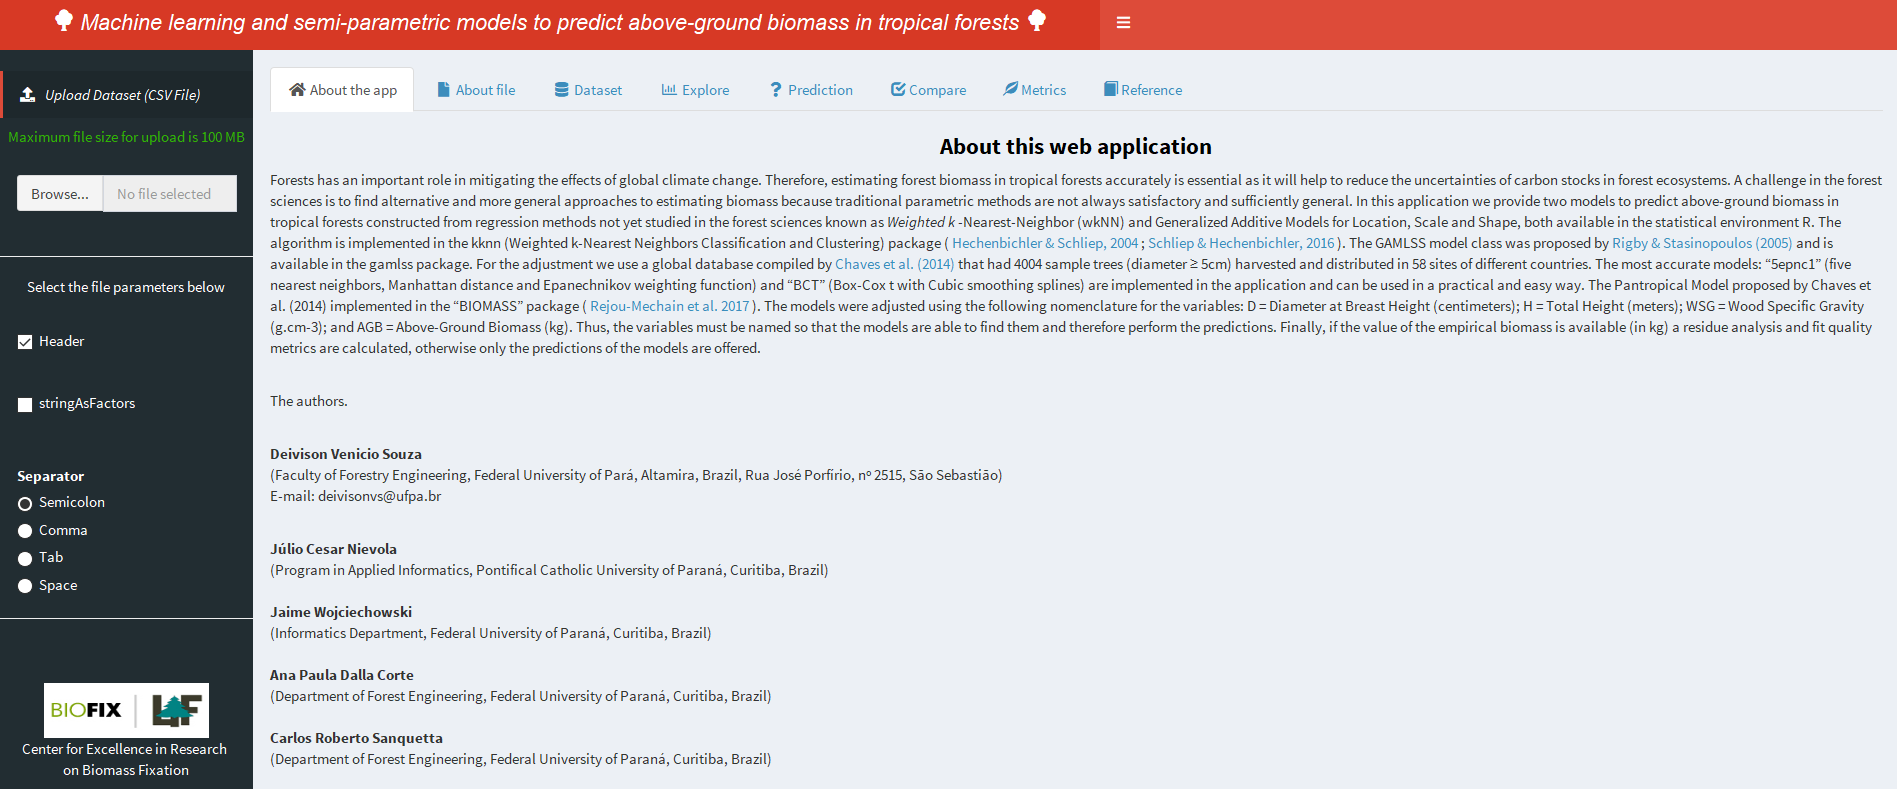
\includegraphics[scale = .35]{Fig/app.png}
	\end{figure}
	
\end{frame}

%%%%%%%%%%%%%%%%%%%%%%%%%%%%%%%%%%%%%%%%%%%%%%%%%%%%%%%%%%%%%%%%%%%%%%%%%%%
% CONSIDERAÇÕES FINAIS
%%%%%%%%%%%%%%%%%%%%%%%%%%%%%%%%%%%%%%%%%%%%%%%%%%%%%%%%%%%%%%%%%%%%%%%%%%%%%%
%\begin{frame}[t]{Considerações Finais}

	%\begin{variableblock}{Desafios}{bg=white,fg=black}{bg=black,fg=white}
	%\justifying
	%\textcolor{blue}{Compreender melhor e avançar} nas implementações de %tarefas de ML nas Ciências Florestais! \\~\\
	%\end{variableblock}
		
	%\begin{variableblock}{Recomendação}{bg=white,fg=black}{bg=black,fg=white}
	%Aprender uma linguagem de programação.
	%\end{variableblock}
		
     %   \begin{center}
      %      
\includegraphics[height=2cm, width=2.5cm]{Fig/R_logo.png}
     %       
\includegraphics[height=3cm, width=5cm]{Fig/python.png}
     %   \end{center}

%\end{frame}

%%%%%%%%%%%%%%%%%%%%%%%%%%%%%%%%%%%%%%%%%%%%%%%%%%%%%%%%%%%%%%%%%%%%%%%%%%%%%%
% CONSIDERAÇÕES FINAIS
%%%%%%%%%%%%%%%%%%%%%%%%%%%%%%%%%%%%%%%%%%%%%%%%%%%%%%%%%%%%%%%%%%%%%%%%%%%%%%
\begin{frame}[t]{Considerações Finais}

    \begin{variableblock}{Aprendizado de Máquina}{bg=white,fg=black}{bg=black,fg=white}
	\justifying
	- \textcolor{blue}{Alternativa potencial} para solucionar problemas florestais mais complexos.
    
    - Linguagem R:
    
    \textcolor{blue}{\textbf{Pacote CAReT}}: Excelente framework para construção de modelos de IA.
    
   \textcolor{blue}{\textbf{Pacote Shiny}}: Uma forma amigável de disponibilizar o modelo de IA para o usuário final.
    
	\end{variableblock}

	\hspace{10cm}\Springtree[2]\Springtree[3]\Springtree[4]\Springtree[5]
\end{frame}

%%%%%%%%%%%%%%%%%%%%%%%%%%%%%%%%%%%%%%%%%%%%%%%%%%%%%%%%%%%%%%%%%%%%%%%%%%%%%%
% BIBLIOGRAFIA
%%%%%%%%%%%%%%%%%%%%%%%%%%%%%%%%%%%%%%%%%%%%%%%%%%%%%%%%%%%%%%%%%%%%%%%%%%%%%%

\begin{frame}[t,allowframebreaks]{Bibliografia}
	\bibliography{refs}
\end{frame}

%%%%%%%%%%%%%%%%%%%%%%%%%%%%%%%%%%%%%%%%%%%%%%%%%%%%%%%%%%%%%%%%%%%%%%%%%%%%%%
%% AGRADECIMENTO
%%%%%%%%%%%%%%%%%%%%%%%%%%%%%%%%%%%%%%%%%%%%%%%%%%%%%%%%%%%%%%%%%%%%%%%%%%%%%%

\begin{frame}[c]{}
	
	\begin{center}
		\textcolor{white}{{\Large \textbf{OBRIGADO!}} \\~\\
		Deivison Venicio Souza (UFPA) \\
		Email: deivisonvs@ufpa.br} \\~\\
		\Springtree[5]
	\end{center}
	
\end{frame}

\end{document}

%%%%%%%%%%%%%%%%%%%%%%%%%%%%%%%%%%%%%%%%%%%%%%%%%%%%%%%%%%%%%%%%%%%%%%%%%%%%%%